\chapter{Installation}\label{chap:install}

This chapter explains step-by-step how to set up a development environment for Harmony.  The Harmony framework is based on the OSGi component model. Even though you may use any OSGi implementation for developing and running your analyses, this documentation shows how to do it with the Equinox implementation developed by the Eclipse community. That is why we use Eclipse as IDE in order to ease the development of new analyses.

\screecast{http://youtu.be/wFGXayQADeA}

\section{Install}



\begin{itemize}
	\item Install Eclipse from \url{http://www.eclipse.org/downloads/}. 
		\begin{itemize}
			\item We recommend {\color{ggreen}\textbf{Eclipse Standard 4.3 (Kepler)}}
			\item No installation support for {\color{gred}\textbf{Eclipse IDE for Java Developers}}
		\end{itemize}
			\item Once downloaded, unzip the Eclipse archive
			\item Run Eclipse
			\item Go to \texttt{Help $\rightarrow$ Install new software}
			\item Click on \texttt{Add...} at the right of the "work with" field
			\item On the popup type:
			\begin{itemize}
				\item \emph{Name}: Harmony
				\item \emph{Location} \url{http://se.labri.fr/data/harmony/update-site}
			\end{itemize}
			\item Click \texttt{OK} and select in the "work with" list the Harmony update site.
			\item Select \texttt{Harmony} on the list (see figure \ref{fig:harmonyInstall})
			\item Click on \texttt{Next}
			\item Accept the terms and click on \texttt{Finish}
			\item If a pop-up with \emph{Security Warning} appears, Click on \texttt{OK}
			\item Restart Eclipse
			\item Harmony is now installed into your Eclipse installation
\end{itemize}



	\begin{figure}[H]
		\centering
		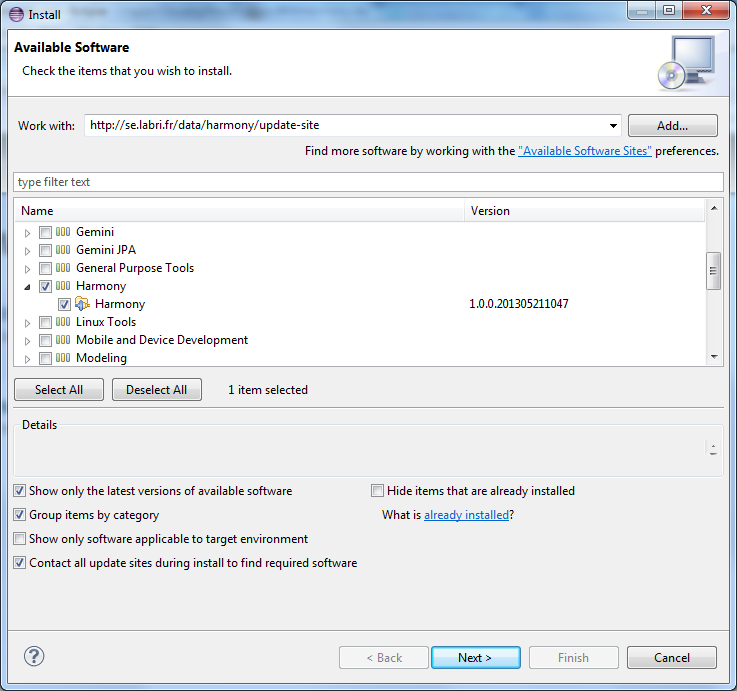
\includegraphics[width=.9\linewidth]{install-harmony}
		\caption{Harmony installation within the Eclipse IDE}
		\label{fig:harmonyInstall}
	\end{figure}



\section{Run}\label{sec:RunInEclipse}

	\begin{itemize}
		\item Go to \texttt{File $\rightarrow$ New $\rightarrow$ Project...}
		\item Select \texttt{WorkingDirectory} under the \texttt{Harmony} category and click on \texttt{Next} (see figure \ref{fig:new-workingdir})
		\item Click on \texttt{Finish}: the wizard will configure your development environment and launch the OSGi console. 
		\item Type \texttt{harmony} in the OSGi console and press Enter (see figure \ref{fig:run-result})
		\item Wait for the harmony analysis to finish. Once done, make a right click on the \emph{WorkingDirectory} project and select \texttt{Refresh}.
		\item If the analysis was successful the folders \emph{tmp} and \emph{out} should appear (see figure \ref{fig:run-result}). You can take a look at the analysis results by looking at the produced files in the \emph{out} directory.
	\end{itemize}
	
	\begin{figure}[H]
		\centering
		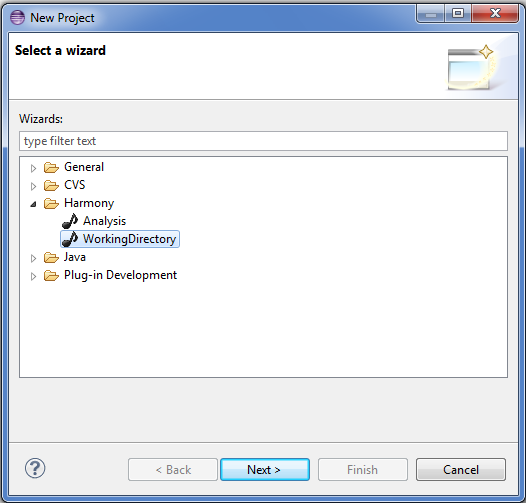
\includegraphics[width=.65\linewidth]{new-workingdir}
		\caption{Selection of the wizard for creating a new working directory}
		\label{fig:new-workingdir}
	\end{figure}
	
	\begin{figure}[H]
		\centering
		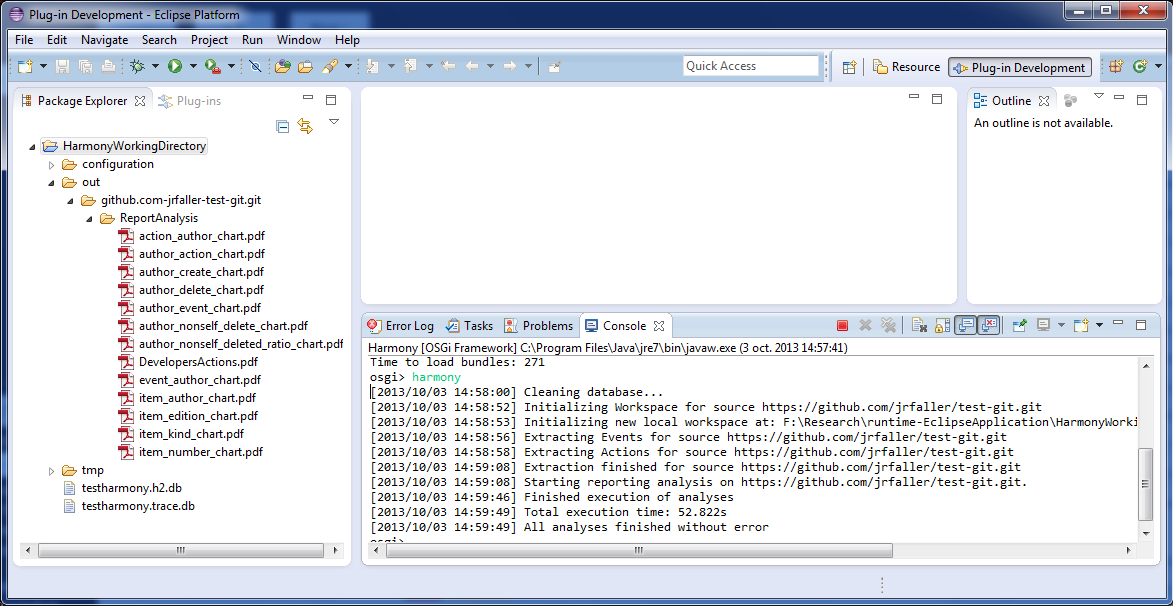
\includegraphics[width=\linewidth]{run-result}
		\caption{Eclipse after the first run of Harmony}
		\label{fig:run-result}
	\end{figure}